\chapter{Einleitung}\label{chapter:einleitung}
%TODO: ADRB2, durchgehend; Skalen; Deckblatt

\section{G-Protein-gekoppelte Rezeptoren (GPCR)}
\label{generalGPCR}
G-Protein-gekoppelte Rezeptoren (GPCRs) stellen die größte Familie der Membranproteine dar. Sie vermitteln zelluläre Antworten auf Hormone und Neurotransmitter, bilden die Rezeptoren des olfaktorischen Systems und können sogar Photonen in zelluläre Signale umsetzen \parencite{Rosenbaum2009}. Allein für das olfaktorische System sind hunderte strukturell verwandter GPCRs bekannt. Damit bilden Moleküle, die GPCRs zum Ziel haben heute die Gruppe der am meisten verwendeten Medikamente \parencite{Pierce2002}.

Alle GPCRs besitzen sieben hydrophobe alpha-helikale Transmembransegmente (7TM-Rezeptoren). Das Aminoende (N-Terminus) ist extrazellulär lokalisiert, das Carboxyende (C-Terminus) intrazellulär. Dazwischen liegen alternierend intra- und extrazelluläre Schleifen. 

Bei beeindruckender funktioneller Diversität lassen sich die GPCRs aufgrund struktureller Homologien in fünf Familien unterteilen \parencite{Fredriksson2003}: Rhodopsin- (Klasse A), Sekretin- (Klasse B), Glutamat- (Klasse C), Adhäsions- (Klasse D) und Frizzled/Taste-Rezeptoren (Klasse E).
Die bei weitem größte unter ihnen bilden die rhodopsinverwandten Rezeptoren (dem "`Lichtrezeptor"' ähnliche Rezeptoren), zu denen auch der in dieser Arbeit näher untersuchte $\beta_2$-adrenerge Rezeptor (ADRB2) gehört.
\subsection{Signaltransduktion}

GPCRs sind in der Lage, stimulatorische (Gs) und inhibitorische guaninnukleotidbindende Proteine (G-Proteine) zu binden, die zu unterschiedlichen Signalkaskaden führen (s. Abb. \ref{fig:gpcr}): 

\begin{figure}[htbp]
	\centering
    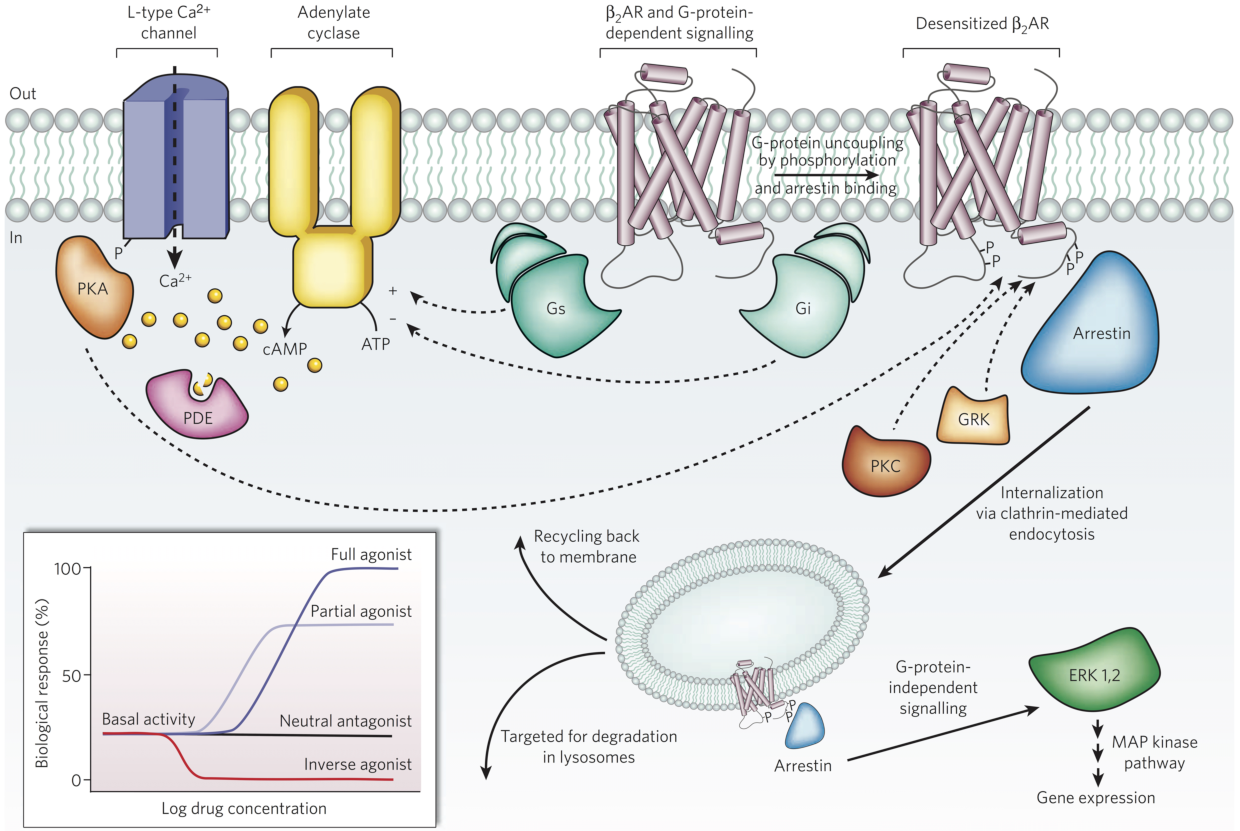
\includegraphics[width=1.0\textwidth]{fig_gpcr.pdf}
    \caption{\textbf{Signaltransduktion eines GPCRs am Beispiel des ADRB2 ($\boldsymbol\beta_2$AR) aus \cite{Rosenbaum2009}}} 
    \label{fig:gpcr}
\end{figure}

Anhand der Funktion des ADRB2 kann die klassische Funktion eines GPCRs illustriert werden: Nach Bindung der natürlichen Agonisten Adrenalin oder Noradrenalin wird die stimulatorische Untereinheit eines heterotrimeren G-Protein aktiviert (G$\alpha$S). Diese führt zur Stimulation der Adenylatzyklase und damit zur Produktion von zyklischem AMP (cAMP). Das akkumulierte cAMP wiederum aktiviert die cAMP-abhängige Proteinkinase A (PKA), die Proteine phosphoryliert und inaktiviert, die für die Kontraktion glatter Muskelzellen verantwortlich sind (L-Typ-Kalziumkanäle) \parencite{Hoffman1982}. 

Die Aktivierung des ADRB2 führt daneben zur Phosphorylierung durch die G-Protein-gekoppelte Rezeptorkinase (GRK). Die Phosphorylierung ermöglicht die Bindung des Proteins Arrestin, das seinerseits als regulatorisches und Signalprotein fungiert. Es deaktiviert den GPCR und führt über Clathrinpits zur endozytotischen Internalisierung des Rezeptors (s. Abschnitt \ref{internalization}), der danach entweder zur Membran recycled oder in Lysosomen degradiert wird. 

Daneben bedingt Arrestin die Aktivierung extrazellulärer signalregulierter Kinasen (ERK 1,2). Diese wiederum regulieren über MAP (mitogen-activated-pathway)-Kinasen die Genexpression.

\section{Adrenerge Rezeptoren}
\subsection{Das $\beta$-adrenerge System}
Die Klasse der adrenergen Rezeptoren umfasst $\alpha$- und $\beta$-adrenerge Rezeptoren. Diese wiederum lassen sich in drei $\alpha_1$-Subtypen ($\alpha_{1A}$, $\alpha_{1B}$, $\alpha_{1D}$), drei $\alpha_2$-Subtypen ($\alpha_{2A}$, $\alpha_{2B}$, $\alpha_{2C}$) sowie in die beiden $\beta$-Subtypen $\beta_1$ und den in dieser Arbeit betrachteten $\beta_2$-Rezeptor unterteilen (\url{http://www.guidetopharmacology.org}).

\subsection{Polymorphismen der $\beta$-adrenergen Rezeptoren}
\label{polymorphisms}
Aufgrund der funktionellen Eigenschaften des ADRB2 ist er häufiges Ziel von Medikamenten, die bei der Behandlung von obstruktiven bronchopulmonalen Erkrankungen eingesetzt werden \parencite{Ortega2007}. Bei der Anwendung von Agonisten des ADRB2 konnten signifikante interindividuelle Unterschiede bei den Ansprechraten gefunden werden \parencite{Hawkins2006}. Als in diesem Zusammenhang bedeutsam konnten mehrere genetische Unterschiede identifiziert werden. So existieren mindestens 49 Single Nucleotide Polymorphismen (SNPs) mit teils unterschiedlichen pharmakologischen und klinischen Eigenschaften \parencite{Chung2011}. %TODO: Varianten
Bereits in älteren Arbeiten konnten in-vitro signifikante Unterschiede bei der Regulation der Expression der polymorphen ADRB2-Varianten nachgewiesen werden \parencite{Green1994}. Die Gly\textsuperscript{16}/Gln\textsuperscript{27}-Variante des ADRB2 zeigte dabei signifikant ausgeprägtere Herabregulation der Expression gegenüber der Arg\textsuperscript{16}/\textsuperscript{27}-Variante. 

\subsection{Rezeptorinternalisierung}
\label{internalization}
Gleichzeitig zur Entdeckung, dass durch Agonisten der $\beta$-adrenergen Rezeptoren ein zellulärer  Signalprozess in Gang gesetzt wird, konnten Veränderungen der Rezeptorendichte auf der Membran gefunden werden \parencite{Chuang1979}. 

\section{Oligomerisierung G-Protein-gekoppelter Rezeptoren}
\subsection{Homo- und Heterooligomerisierung G-Protein-gekoppelter Rezeptoren}
Die klassische Annahme, GPCRs würden als monomere Proteine funktionieren, konnte durch eine große Zahl unterschiedlicher Studien widerlegt werden. Tatsächlich sind nach zahlreichen BRET- und FRET-gestützten Untersuchungen mittlerweile sowohl Hetero- als auch als Homodimere einer Vielzahl von GPCRs bekannt (\cite{Khelashvili2010}, \url{http://www.gpcr-okb.org}).

Als Reaktion auf die stetig wachsende Informationen über Rezeptoroligomerisierung veröffentlichte die International Union of Basic and Clinical Pharmacology (IUPHAR) drei Kriterien, von denen mindestens zwei erfüllt sein sollen, um die physiologische Relevanz der Oligomere einordnen zu können \parencite{Pin2007}. Die drei Kriterien umfassen:
\begin{enumerate}
\item Den Nachweis der physischen Interaktion der am Oligomer beteiligten Rezeptoren in nativem Gewebe oder primären Zellen. Dabei wird hinreichende methodische Sicherheit gefordert: Bloße Co-Immunopräzipitationsstudien genügen beispielsweise nicht für den überzeugenden Nachweis physischer Interaktion.
\item Funktionelle oligomerspezifische Besonderheiten wie positive oder negative allosterische Interaktion oder auch den Nachweis eines oligomerspezifischen Liganden (s. Abschnitt \ref{drugs}). Auch der Nachweis einer spezifisch durch den Oligomer modifizierten Signalskaskade kann an dieser Stelle stehen.
\item Validierung des Rezeptoroligomers in-vivo mittels beispielsweise Knock-Out-Mäusen oder RNAi-basierten Methoden - unter der Voraussetzung, dass in heterologen Expressionssystemen bereits hinreichende Relevanz bestätigt werden konnte. 

\end{enumerate}
Für einige Steroidrezeptoren und Rezeptoren mit Tyrosinkinaseaktivität ist die Rolle ihrer Oligomerisierung seit längerer Zeit etabliert \parencite{Heldin1995}. Im Falle der GPCRs ist die Existenz der Rezeptoroligomere heute in vielen Fällen akzeptiert, doch führt die Bewertung ihrer funktionellen Bedeutung weiter zu kontroversen Diskussionen - etwa weil sich die meisten Untersuchungen heterologer Expressionssysteme bedienten, die beispielsweise Rezeptoren exprimierten, die in-vivo nicht gemeinsam exprimiert werden. Zum anderen wird weiter diskutiert, welche Untereinheiten der Rezeptoren tatsächlich das Interface der beobachteten Rezeptoroligomere bilden \parencite{Terrillon2004}. 

Ebenso bleibt Gegenstand der Diskussion, wie viele Rezeptoren in einem Oligomer gruppiert sind. Häufiger taucht die These auf, Dimere seien die vorherrschende stöchiometrische Einheit \parencite{Dorsch2009}, erst mit steigender Expressionstärke ergäben sich höhergradige Oligomere \parencite{Calebiro2013}. Gleiches konnte für den GABA\textsubscript{B}-Rezeptor beobachtet werden \parencite{Maurel2008, Comps-agrar2011}. Untersuchungen, die sich der Fluorescence-Correlation-Spectroscopy (FCS) und Photon-Counting-Histogram (PCH) bedienen, deuten ebenfalls darauf hin, dass Dimere bei mehreren GPCRs die funktionelle Einheit bilden \parencite{Herrick-Davis2013}. In der vorliegenden Arbeit wird der Begriff "`Oligomere"' bei weiter nicht vollständig geklärter Stöchiometrie bevorzugt, da die wahrscheinliche Dimer-Konfiguration einen Spezialfall des allgemeineren Begriffes darstellt.
\\ \\
Rezeptoroligomere haben eine Reihe denkbarer Implikationen. Fünf postulierte und beobachtete Rollen der Rezeptoroligomerisierung sind in Abbildung \ref{fig:lifecycle} illustriert:

\begin{figure}[htbp]
	\centering
    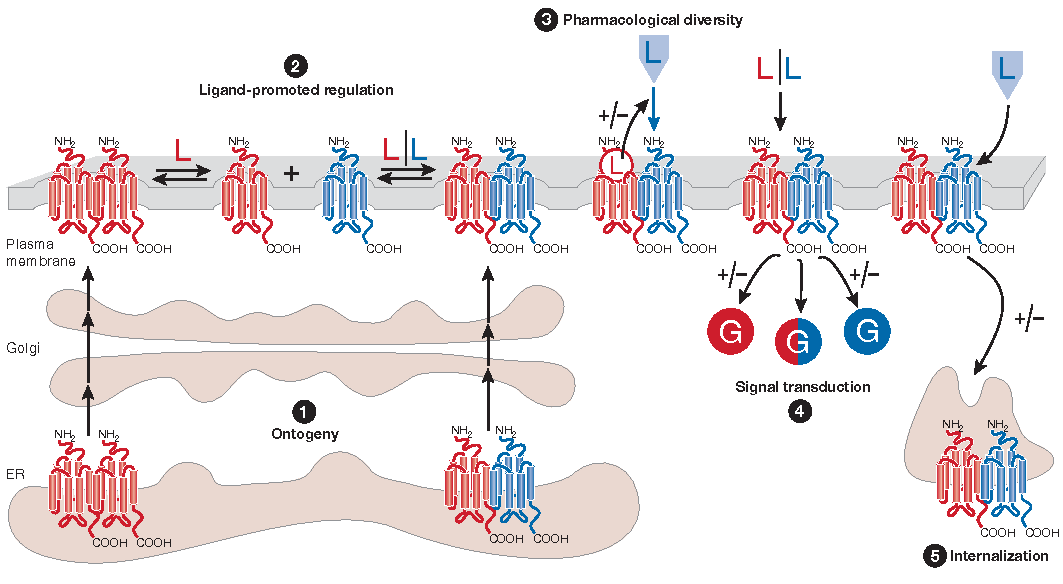
\includegraphics[width=1.0\textwidth]{fig_lifecycle.pdf}
    \caption{\textbf{Rolle der Rezeptoroligomerisierung (aus \cite{Terrillon2004}):} 1 Rezeptorreifung; 2 Dynamische Regulierung der Oligomerisierung durch Ligandenbindung; 3 Heterodimerisierung von Rezeptoren bedingt positiv- oder negativ-kooperative Ligandenbindung; 4 verstärkte und inhibierte Signaltransduktion als Folge der Rezeptoroligomerisierung; 5 Heterooligomerisierung ruft möglicherweise Rezeptorinternalisierung schon bei Aktivierung nur eines Protomers hervor beziehungsweise blockiert ein endozytoseresistenter Protomer die Internalisierung seines gekoppelten Rezeptors im Heterooligomer} 
    \label{fig:lifecycle}
\end{figure}
\begin{itemize}
\item So sind Biosynthese und korrekte posttranslationale Modifikationen im endoplasmatischen Retikulum (ER) möglicherweise Voraussetzung für Integration in die Zellmembran \parencite{Salahpour2004}. Wurden GPCRs mit einem Retentions-Signal versehen, das den Export aus dem Endoplasmatischen Retikulum verhinderte, bedingte dies die Retention des untersuchten Heterooligomers \parencite{Zhu1998, Lee2000, Issafras2002, Floyd2003}.
\item Im Falle des Heterooligomers aus $\mu$- und $\delta$-Opioid-Rezeptoren wurde beobachtet, dass die Bindung eines für den einen Rezeptor spezifischen Liganden über Beeinflussung der Rezeptorkonfirmation die Affinität für den Agonisten des anderen verstärkt \parencite{Gomes2004}. Ein Phänomen, das als positive Kooperativität bezeichnet wird.
\item Auf der Ebene der durch G-Proteine vermittelten Signalkaskade (s. Abschnitt \ref{generalGPCR}) konnte für die Dopaminrezeptoren D1 und D2 im Heterooligomer veränderte Bindungseigenschaften gegenüber dem Gq/11-Protein und somit veränderte Signaleigenschaften gemessen werden \parencite{Rashid2007}.
\item Schließlich konnte gezeigt werden, dass Rezeptorinternalisierung eines Protomers im Fall von Heterooligomeren effektiv auch zur Internalisierung des anderen führen, beziehungsweise diese verhindern kann \parencite{Hillion2002, Milligan2010, Ward2011}. 
\end{itemize}

\subsection{Physiologische Relevanz von Rezeptoroligomeren}
In einer Reihe von Pathologien konnte eine Bedeutung von Rezeptoroligomerisierung im Zusammenhang mit den oben genannten Mechanismen identifiziert werden:
\\ \\
In der Asthmatherapie spielen beispielsweise Agonisten des ADRB2 als Bronchodilatatoren eine führende Rolle. In einer Publikation von \cite{McGraw2006} wurde ein Cross-Talk zwischen dem Prostanoid-Rezeptor EP1 (EP1R) und dem ADRB2 gezeigt: Prostaglandin E2 (PGE2) führte zu verstärkter Dimerisierung des EP1R und des ADRB2 - mit geringerer cAMP-Produktion als Zeichen verminderter ADRB2-Aktivierung.

Bei Patienten mit Major-Depression wurde der Anteil oligomerisierter D1- und D2-Rezeptoren in post-mortem-Studien mittels Co-Immunopräzipitation signifikant erhöht gegenüber gesunden Probanden gemessen \parencite{Pei2010}. Möglicherweise können in Zukunft Medikamente, die die Oligomerisierung der beiden Rezeptoren beeinflussen, therapeutische Bedeutung für die Depression gewinnen. 

In mehreren Untersuchungen, unter anderem mit bivalenten Liganden (s. Abschnitt \ref{drugs}), wurde dem Heterooligomer aus $\delta$- und $\mu$-OR negative Kooperativität in-vivo beigemessen \parencite{Daniels2005, Lenard2007, He2011}. Ähnlich wie bei beim Dopaminrezeptor im Falle der Depression könnte Beeinflussung der Oligomerisierung von pharmakologischer Relevanz werden.
\\ \\
Weitere physiologisch bedeutsame Konstrukte konnten bei der Parkinson-Erkrankung \parencite{Tanganelli2004, Fuxe2003, Fuxe2005} sowie bei Prä-Eklampsie (Hypertonie) \parencite{AbdAlla2001} gefunden werden.

\subsection{Rezeptoroligomere als Targets neuartiger Wirkstoffe}
\label{drugs}
GPCR-Heterooligomere stellen bisher nicht adressierte Angriffspunkte für eine neue Klasse von Arzneimitteln dar \parencite{George2002, Hiller2013, Ferre2014}. Denkbar ist die Entwicklung neuer Substanzen, die aufgrund höherer Selektivität und Affinität weniger unerwünschte Wirkungen aufweisen. Hinweise für gewebsspezifische Heterooligomere bleiben Gegenstand der aktuellen Forschung. 

Prinzipiell können mono- und bivalente Liganden, d.h. Substanzen, die aus einem oder zwei bekannten GPCR-Liganden bestehen eingesetzt werden, um selektive Affinität für Oligomere zu erreichen \parencite{Waldhoer2005, Burford2014}. Die Synthese birgt dabei einige Schwierigkeiten, da die chemischen Eigenschaften zum Teil erheblich von denen der Einzelliganden abweichen \parencite{Hiller2013}. Eine Tatsache, die auch bei den fluoreszierenden Liganden, die in dieser Arbeit verwendet wurden zu untersuchen war.

Neben den klassischen orthosterischen Liganden seien die Möglichkeiten allosterischer Liganden erwähnt. 

In einer Studie von \cite{Waldhoer2005} zeigte beispielsweise ein monovalenter Ligand (6'-GNTI) bevorzugte Aktivierung des Heterodimers aus $\delta$- und $\kappa$-OR. In-vivo bewirkte der Ligand bei intrathekaler Gabe Analgesie, nicht jedoch bei intrazerebroventrikulärer Gabe, was eventuell auf Gewebsspezifität hinweist.
\\ \\
Mittlerweile sind eine Reihe bivalenter Liganden synthetisiert worden, die unter anderem Serotonin-, Histamin-, Dopamin-, Adenosin- Chemokin-, Cannabinoid-, Muskarin- und auch adrenerge Rezeptoren zum Ziel haben \parencite{Hiller2013}. Welche Substanzen in Zukunft von Bedeutung sein werden, bleibt zu diskutieren.

\section{Methoden zur Untersuchung der Oligomerisierung von Rezeptoren}
\subsection{Überblick}
Es existieren eine Vielzahl von Methoden, die zum Nachweis von Rezeptoroligomerisierung verwendet worden sind. Die am häufigsten und aktuell verwendeten werden im folgenden dargestellt, um auf die Zielsetzung dieser Arbeit hinzuleiten.

\subsubsection {Co-Immunopräzipitation}
Eine der am häufigsten verwendeten Methoden stellt die Co-Immunopräzipitation dar \parencite{Hebert1996, Jordan1999, Hillion2002, Park2004}. In der einfachsten Variante mit einem Protein-Epitop-tag und dem passenden spezifischen Antikörper war aufgefallen, dass die untersuchten Rezeptoren jeweils in den Banden ganzzahliger Vielfacher des Molekulargewichts liefen. Der Vermutung, es könnte sich um Oligomere handeln, liegt nahe. Allerdings konnte so nicht ausgeschlossen werden, dass es sich um unspezifische Rezeptor-Protein-Aggregate handelte. Genauer gelang der Nachweis mithilfe zweier Protein-Epitop-tags und zwei spezifischen Antikörpern. So konnten untersuchte Rezeptoren erst immunpräzipitiert und anschließend mit dem zweiten Antikörper geblottet werden.

\subsubsection{Kristallstrukturen oligomerisierter Rezeptoren}
Eine direkte Nachweismöglichkeit oligomerisierter Rezeptoren bietet die aufwändige Gewinnung der Kristallstruktur der Rezeptoren. Im Falle des CXCR4-Chemokin-Rezeptors und der Opioid-Rezeptor-Subtypen $\mu$OR und $\kappa$OR konnten in den Kristallstrukturen strikte Rezeptordimere beobachtet werden \parencite{Wu2010, Manglik2012, Wu2012}. Die mit dieser Methode identifizierten Oligomerisierungsinterfaces waren für die jeweiligen Rezeptoren unterschiedlich lokalisiert und werden in Zukunft Gegenstand weiterer Analysen werden.

\subsubsection{Fluoreszenz-basierte Methoden}
Fluoreszenz-basierte Methoden zur Analyse der Oligomerstruktur von GPCRs bedienen sich dem Resonanzenergietransfer (RET) zwischen biolumineszenten oder synthetischen Fluorophoren. In Abschnitt \ref{ret} sind die Methoden genauer dargestellt.

\subsubsection{Funktionelle Untersuchungen}
Weitere, insbesondere für in-vivo-Untersuchungen essentielle Verfahren, schließen über funktionelle Analyse indirekt auf die Existenz oligomerisierter Rezeptoren. Sie bedienen sich etwa bivalenter Liganden \parencite{Daniels2005} oder elektrophysiologischer Untersuchungen der G \textsubscript{i}- beziehungsweise G\textsubscript{q}-Protein-assoziierten Signalwege \parencite{Fribourg2011a}.
 
\subsection{BRET \& FRET zur Analyse oligomerisierter Rezeptoren}
\label{ret}

Am häufigsten kommen \gls{bret} und \gls{fret} zum Einsatz. In beiden Fällen bedient man sich einem Effekt, der als Resonanzenergietransfer bekannt ist: Dabei kommt es bei Exzitation eines Donorfluorophors zu dipolvermitteltem, strahlungsfreien Energietransfer auf einen Akzeptor, wenn sich die beiden beteiligten Fluorophore in geeignetem Abstand (Förster-Radius) zueinander befinden. Nach dem Energietransfer emittiert dann im Idealfall nur das Akzeptorfluorophor ein Photon seiner (größeren) Wellenlänge \parencite{Forster1948}. Alternativ lässt sich stattgehabter Resonanzenergietransfer auch als Verringerung der Intensität, Länge oder als Anisotropie der Donoremission messen \parencite{Rajapakse2010}.

Dieser Effekt kann nun verwendet werden, um die räumliche Nähe im Bereich der Förster-Radien beliebiger Strukturen zu zeigen. Die notwendige Entfernung liegt üblicherweise bei $d<10$\si{\nano\meter}. 

Bei BRET-basierten Analysen werden Fusionsproteine generiert, die C-terminal über ein biolumineszentes Protein, beispielsweise Renilla-reniformis-Luciferase (Rluc) als Donor und fluoreszente Proteine wie YFP als Akzeptor verfügen \parencite{Pfleger2006}. Die subzelluläre Lokalisation ist mit diesem Ansatz nicht eindeutig bestimmbar. Außerdem bietet die Methode geringere Signalausbeute als auf synthetischen Fluorophoren basierende Methoden.
\\ \\
Der Übersicht halber werden weitere, für speziellere Anwendungen benötigte Methoden kurz erläutert:

Die Fluorescence-Recovery-After-Photobleaching-(FRAP)-Methode ist eine ebenfalls fluoreszenzbasierte Methode, die sich nicht dem Resonanzenergietransfer bedient. Nach antikörpervermittelter Immobilisation beispielsweise einer Rezeptorfraktion werden die Fluorophore, die sich auf einem definierten Membranabschnitt befinden durch lange Exzitation geblichen. Anschließend wird die Repopulation als Maß der Rezeptoroligomerisierung gedeutet \parencite{Dorsch2009}.

%FRET-Mikroskopie

\begin{figure}[htbp]
	\centering
    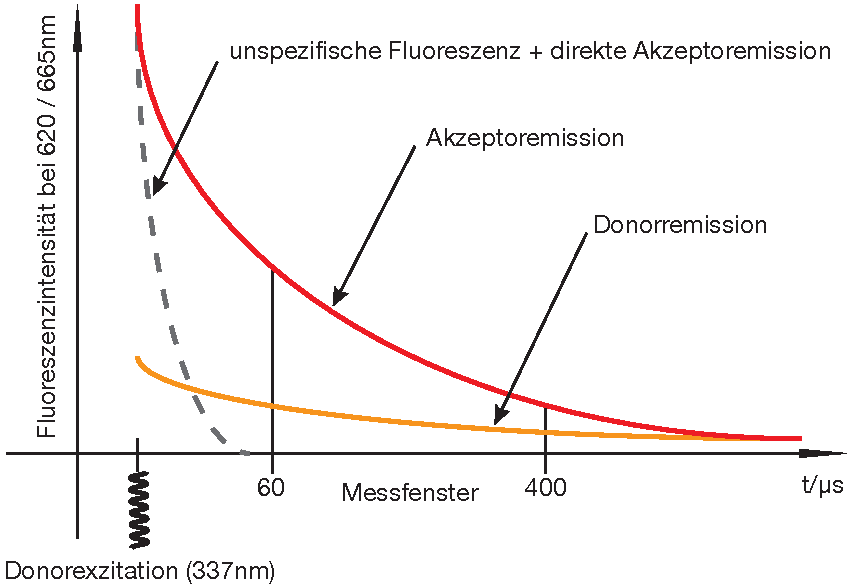
\includegraphics[width=0.8\textwidth]{fig_trfret.pdf}
    \caption{\textbf{Funktionsprinzip der tr-FRET-Methode:} Die Messung der Akzeptoremmission erfolgt erst 60\si{\nano\second} nach Exzitation des Donors. So können die Störsignale der kurzlebigen unspezifische Matrixfluoreszenz und direkte Exzitation des Akzeptors durch den initialen Energiepuls minimiert werden.} 
    \label{fig:trfret}
\end{figure}

\subsubsection{Time-resolved FRET (tr-FRET)}
Die in dieser Arbeit verwendete Technik (tr-FRET) bietet gegenüber den zuvor erläuterten Methoden mehrere Weiterentwicklungen.

Bei der tr-FRET-Methode wird als Donor ein in einem Chelatkomplex gebundenes Lanthanid (beispielsweise Terbium- oder Europium) verwendet. Genaugenommen handelt es sich bei der Lanthanidemission nicht um Fluoreszenz, sondern um eine physikalisch anderes begründete Strahlung (Singulett-Singulett-Zustandsübergang). Die Lanthanide bieten gegenüber synthetischen oder biolumineszenten Proteinen zum einen deutlich länger anhaltende Emission im Milllisekundenbereich und zum anderen einen breiten Stokes-Shift (Wellenlängendifferenz zwischen Exzitation und Emission) bei äußerst schmalem Emissionsspektrum \parencite{Selvin1994, Selvin2002}.

Beim tr-FRET kann nun die Messung der Akzeptoremission zeitversetzt zur Exzitation des Donors erfolgen. Das Prinzip ist in Abbildung \ref{fig:trfret} dargestellt: Erst nachdem die kurzlebige Autofluoreszenz (bereits nach weniger als 100\si{\nano\second}) und direkte Exzitation des Akzeptors größtenteils verschwunden sind \parencite{Selvin2002}. 

Damit lässt sich das Verhältnis zwischen Signal und Hintergrund auf ein Niveau anheben, das ausreichend sein kann, Rezeptoroligomere in natürlich vorkommender Expressionsstärke nachzuweisen \parencite{Albizu2010}.
\\ \\
Limitiert ist die Methode in Bezug auf den Nachweis der Anzahl der sich in einem Oligomer befindenden Protomere (s. Abschnitt \ref{discussion:limits}). 

%FRAP?
\subsubsection{Proteinlabeling mit dem SNAP-tag}
Zur spezifischen Adressierung von Proteinen wie den GPCRs existieren eine Reihe unterschiedlicher Systeme. Dazu zählen Verfahren wie das Proximity Ligation Assay (PLA) \parencite{Soderberg2006} oder  N-Terminale tags wie der Flag-tag, die sich auf strukturell große Antikörper stützen. 

Daneben können tag-Systeme mit intrinsischer Enzymaktivität verwendet werden, um spezifische kovalente Bindungen mit den gewünschten Proteinuntereinheiten zu katalysieren \parencite{Gautier2008}. Das in dieser Arbeit verwendete Prinzip beruht auf einem Proteinlabelingsystem, das es erlaubt, Fluorophore kovalent an ein N-terminal lokalisiertes Fusionsprotein zu koppeln. Mittels eines mutierten DNA-Reparaturenzyms erfolgt die kovalente Bindung des tr-FRET-Fluorophors (s. \ref{klonierung}). Dazu müssen die zu untersuchenden Proteine vor weiterer Charakterisierung jedoch zuerst um die Fusionsproteine erweitert werden, die die gewünschte Enzymaktivität besitzen. Es ist ersichtlich, dass mit dieser Methode allein in primären Zellen noch kein Nachweis gelingen kann.

\subsubsection{Nachweis von GPCR-Oligomeren mit fluoreszierenden Liganden}
Mit einem komplizierteren Ansatz besteht die Möglichkeit, GPCRs mittels fluoreszierender Liganden auf ihre räumliche Nähe zu untersuchen. Fluoreszierende Liganden bieten den entscheidenden Vorteil, auch für nicht modifizierte, natürlich exprimierte Rezeptoren verwendet werden zu können. Es konnte bereits gezeigt werden, dass mit fluoreszierenden Liganden bei ausreichend hoher Expressionsstärke tr-FRET auch in primären Zellen beziehungsweise Gewebsstücken gemessen werden kann \parencite{Albizu2010}.

\section{Zielsetzung dieser Arbeit}
Ziel dieser Arbeit war, die strukturelle Eigenschaft der Oligomerisierung des ADRB2 zu untersuchen. Dabei sollte die Methode des SNAP-tags in Kombination mit einer hochsensitiven trFRET-gestützten Methode zuerst zur prinzipiellen Untersuchung an transfizierten Zelllinien etabliert werden. Dabei waren mögliche Modulatoren des Oligomerisierungsverhaltens in funktionelle Studien miteinzubeziehen. In einem nächsten Schritt sollten mittels fluoreszierender Liganden der native ADRB2 auf seine Oligomerisierungseigenschaften geprüft werden. Schließlich war die Methode so weit zu optimieren, dass sie zukünftig für in-vivo-Untersuchungen etwa an Gewebsstücken verwendet werden könnte.

Als grundlagenorientierte Arbeit sollte diese Arbeit sich mit strukturell bedeutsamen Prinzipien befassen, die gegenwärtig Gegenstand der Arzneimittelforschung werden.  
